%%%%%%%%%%%%%%%%%%%%%%%%%%%%%%%%%%%%%%%%%%%%%%%%%%%%%%%%%%%%%%%%%%%
%% chapter1.tex
%% UNL thesis document file
%%
%% Chapter with introduciton
%%%%%%%%%%%%%%%%%%%%%%%%%%%%%%%%%%%%%%%%%%%%%%%%%%%%%%%%%%%%%%%%%%%
\newcommand{\unlthesis}{\emph{unlthesis}}
\newcommand{\unlthesisclass}{\texttt{unlthesis.cls}}


\chapter{Introdução}
\label{cha:introdução}

%\begin{quotation}
%  \itshape
%  This work is licensed under the Creative Commons Attribution-NonCommercial~4.0 International License.
%  To view a copy of this license, visit \url{http://creativecommons.org/licenses/by-nc/4.0/}.
%\end{quotation}

\section{Uma curta apresentação} % (fold)
\label{sec:uma_curta_apresentação}

Ao longo dos anos, o número de automóveis existentes nas estradas Portuguesas tem vindo a aumentar constantemente, bem como o número de defeitos e falhas nessas mesmas vias. De modo a caminhar em direção à resolução deste problema, surgiu a oportunidade de realizar o projeto aqui apresentado, em que é sugerida uma das muitas soluções possíveis, utilizando uma abordagem que está diretamente ligada ao rápido aumento de utilizadores de telemóvel bem como ao grande número de condutores em Portugal, visto que existem cerca de 19 milhões de telemóveis em Portugal\footnote{http://www.pordata.pt/Portugal/Assinantes+++equipamentos+de+utilizadores+do+servi\%C3\%A7o+m\%C3\%B3vel-1180} para os cerca de 11 milhões de habitantes na mesma região\footnote{http://www.pordata.pt/Portugal/Popula\%C3\%A7\%C3\%A3o+residente+total+e+por+grupo+et\%C3\%A1rio-10}.

Surge então a necessidade de uma monitorização das vias de trânsito para a sua manutenção e reparação. Desta forma, tentando aliar a tecnologia com este fator, será desenvolvido um sistema que irá ser integrado em automóveis e que possa fazer a deteção e comunicação de defeitos nas estradas em que cada automobilista circula.

Este documento irá fornecer, da forma mais detalhada possível, como construir e montar um sistema de deteção de defeitos nas estradas, utilizando um acelerómetro e um telemóvel, bem como comunicação \emph{bluetooth} e \emph{wi-fi}, de modo a estabelecer a comunicação entre os vários componentes do sistema. Serão também apresentados os diversos pontos fortes e fracos da solução tomada, fazendo sempre a comparação com projetos já desenvolvidos e as suas respetivas soluções.

\section{Descrição de especificações}
\label{sec:descrição_de_especificações}

\subsection{Acelerómetro}
\label{subsec:acelerometro}
		Um acelerómetro é um dispositivo eletromagnético que mede forças de aceleração. Estas forças podem ser constantes ou variáveis, como a força da gravidade ou uma mudança de direção do acelerómetro, respetivamente. Medindo a aceleração gravítica, é possível saber se um automóvel está a subir ou a descer e medindo uma aceleração variável é possível detetar quando um condutor passa por um buraco na estrada. Os acelerómetros podem apresentar diversos modos de funcionamento, que não se vão mostrar relevantes para a execução deste projeto. O que vai ser tido em conta são as funcionalidades que cada um pode apresentar, nomeadamente o número de eixos a medir, a variação máxima das forças que nele são aplicadas e a sua sensibilidade em relação às forças medidas.
\begin{figure}[htbp]
	\centering
	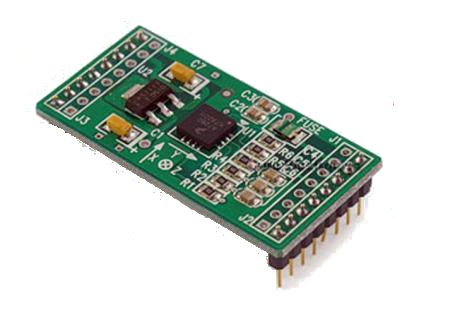
\includegraphics[height=8cm]{acelerometro}
	\caption{Módulo acelerómetro}
	\label{fig:modulo_acelerometro}
\end{figure}	

\subsection{Bluetooth}
\label{subsec:bluetooth}
		Bluetooth é uma tecnologia padrão para comunicações sem fios à escala global que liga dispositivos que se encontrem separados por curtas distâncias e encontra-se integrada em biliões de produtos no mercado atual, fazendo a ligação à Internet das Coisas (Internet of Things). Esta tecnologia utiliza pouca energia e cria uma pequena rede ad hoc que emparelha dois a oito dispositivos remotamente através de um pequeno circuito que comunica utilizando ondas rádio, sendo possível conectar produtos como colunas, luzes, televisões, garrafas de água ou até brinquedos.		
\begin{figure}[htbp]
	\centering
	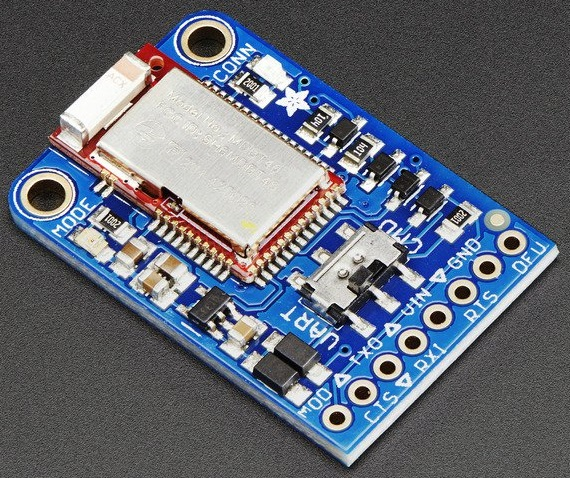
\includegraphics[height=8cm]{bluetooth}
	\caption{Módulo bluetooth}
	\label{fig:modulo_bluetooth}
\end{figure}

\subsection{Wi-fi}
\label{subsec:wi-fi}
		Wi-fi, abreviatura de Wireless Fidelity (fidelidade sem fios) é uma tecnologia que utiliza ondas rádio para fornecer ligação a uma rede e é estabelecida utilizando adaptadores sem fios para criar ponto de acesso (hotspot) que permite aos utilizadores obterem ligação ao serviço de internet, desde que estejam ligados a ele. É necessário um adaptador sem fios para transmitir o sinal via rádio, que é enviado para um descodificador (router) através de uma antena para que toda a informação possa ser enviada via internet, utilizando várias frequências que permitem diversas velocidades de transmissão.
\begin{figure}[htbp]
	\centering
	
\includegraphics[height=8cm]{wifi}
	\caption{Módulo wifi}
	\label{fig:modulo_wifi}
\end{figure}